\chapter{Bayesian Decision Theory}
We are not yet to the point of taking decision. Bayesian decision \textit{theory} allows to take optimal decisions in a fully probabilistic way. \newline
It allows to provide an upper bounds on achievable errors and evaluate classifiers accordingly. Moreover bayesian reasoning can be generalized to cases when the probabilistic structure is not entirely known. \newline
From now on we will be using $P(x)$ for mass functions and $p(x)$ for distribution functions or unknowns.\newline
%
%
\section{Bayes decision Rule}
Let's consider a binary classification. Assume of having examples $(x,y)\in\mathcal{X}\times\{-1,1\}$ drawn from a known distribution $p(x,y)$. The task is predicting the class $y$ of examples given the input $x$, which can be done via Bayes' rule (Definition~\ref{def:BayesRule}):
\begin{center}
	$\displaystyle P(y\vert x)=\cfrac{p(x\vert y)P(y)}{p(x)}$
\end{center}
Bayes rule allows to compute the posterior probability given likelihood, prior and evidence:
\begin{center}
	$\displaystyle \text{posterior}=\cfrac{\text{likelihood}\times\text{prior}}{\text{evidence}}$
\end{center}
Where:
\begin{itemize}
	\item \textbf{posterior} $P(y\vert x)$ is the probability that the class is $y$ given that $x$ was observed;
	\item \textbf{Likelihood} $p(x\vert y)$ is the probability of observing $x$ given that its class is $y$;
	\item \textbf{Prior}: $P(y)$: is the prior probability of the class, without any evidence;
	\item \textbf{Evidence}: $p(x)$ is the probability of the observation, and by the law of total probability -sum rule (Definition~\ref{def:LawTotalProbability}), and the product rule (Definition~\ref{def:ProductRule}), it can be computed as:
\begin{center}
	$\displaystyle p(x)=\Sum_{i=1}^2p(x\vert y)P(y)$
\end{center}
\end{itemize}
When taking decision it's possible to commit mistake, for this reason we want to know the probability of making mistakes. \newline
The probability of an error can be expressed as the probability of the error given $x$ on all possible values of $y$. For example when considering the binomial, then
\[P(error\vert x)=
\begin{cases}
	P(y_2\vert x)\quad \text{if we decide }y_1\\
	P(y_1\vert x)\quad \text{if we decide }y_2\\
\end{cases}
\]
For the sum rule (Definition~\ref{def:SumRule}), the average €error can be expressed as:
\begin{center}
	$\displaystyle P(error)=\Sum_xP(error, x)$
\end{center}
And by the product rule (Definition~\ref{def:ProductRule}), it can be expanded to:
\begin{center}
	$\displaystyle P(error)=\Sum_xP(error\vert x)p(x)$
\end{center}
This is for the discrete case, if the variable were to be continuous, then the formula would be:
\begin{center}
	$\displaystyle P(error)=\int_{-\infty}^\infty P(error\vert x)p(x)dx$
\end{center}
Based on the error probability value, a decision can be made in order to minimize the error maximize the probability of success. This rule is called Bayes Decision Rule and is divided in two cases; the first one is for binary classification:
\begin{equation}
	y_B=\argmax{y_i\in\{-1,1\}}P(y_i\vert x)=\argmax{y_i\in\{-1, 1\}}p(x\vert y_i)P(y_i)
	\label{eq:BayesianDecisionRuleBinary}
\end{equation} 
Mind that by the Bayes Rule (Definition~\ref{def:BayesRule}) the last expression should have $p(x)$ at the denominator, but this doesn't change with the changing of $y_i$, hence it can be removed. \newline
A second case is the multiclass case:
\begin{equation}
	y_B=\argmax{y_i\in\{1, \hdots, c\}}P(y_i\vert x)=\argmax{y_i\in\{1, \hdots, c\}}p(x\vert y_i)P(y_i)
	\label{eq:BayesianDecisionRuleMulticlass}
\end{equation}
The \textbf{optimal rule} says that the probability of error given $x$:
\begin{center}
	$\displaystyle P(error\vert x)=1-P(y_B\vert x)$
\end{center}
Hence, the Bayes Decision Rule \textit{minimizes} the probability of error.\newline
%
%
%
\section{Representing Classifiers}
So when we are making a decision, that is trying to classify an input, we are trying to maximize the probability a posteriori. To execute the classification, a \textit{classifier} is used, that is a function, or more that we hope are as similar to the reality as they can be. \newline
A classifier can be represented as a set of \textbf{discriminant functions} $g_i(\vect{x}), i\{\in1,\hdots,c\}$, where $c$ is the number of classes. For such reason, the Bayes optimal rule can be rewritten as:
\begin{center}
	$\displaystyle y=\argmax{i\in\{1,\hdots, c\}}g_i(\vect{x})$
\end{center}
By comparison with Equation~\ref{eq:varianceNotLinear2}, we have:
\begin{center}
\begin{tabular}{rl}
	$\displaystyle g_i(\vect{x})=$&$P(y_i\vert \vect{x}=\cfrac{p(\vect{x}\vert y_i)P(y_i)}{p(\vect{x})}$\\
	$=$&$p(\vect{x}\vert y_i)P(y_i)$
\end{tabular}
\end{center}
Which by the rule of logarithms can be rewritten as:
\begin{center}
	$\displaystyle g_i(\vect{x})=\ln{p(\vect{x}\vert y_i)}+\ln{P(y_i)}$
\end{center}
With these discriminant functions, the features space is divided into decisions regions $\mathcal{R}_1,\hdots,\mathcal{R}_c$ such that:
\begin{center}
	$\displaystyle \vect{x}\in\mathcal{R}_i\quad \text{if }g_i(\vect{x})>g_j(\vect{x})~\forall j\neq i$
\end{center}
\textbf{Decision regions} are separated by \textbf{decision boundaries}, that is regions in which ties occur among the the discriminant functions and hence the classifier is ambiguous. \newline
Let's suppose to have two features ($\omega_1$ and $\omega_2$) and to divide the space via two discriminant functions, hence binary. The most common choice to model likelihood is using gaussians which allows to have a multivariate normal distribution. From Figure~\ref{fig:BayesDecisionRuleFig1} it's possible to notice the gaussians functions which has two peaks which represents the values for which the class will be chosen. For some values of $x$, the value of $g$ will be the same, hence the decision boundaries. 
\begin{figure}[htp]
	\centering
	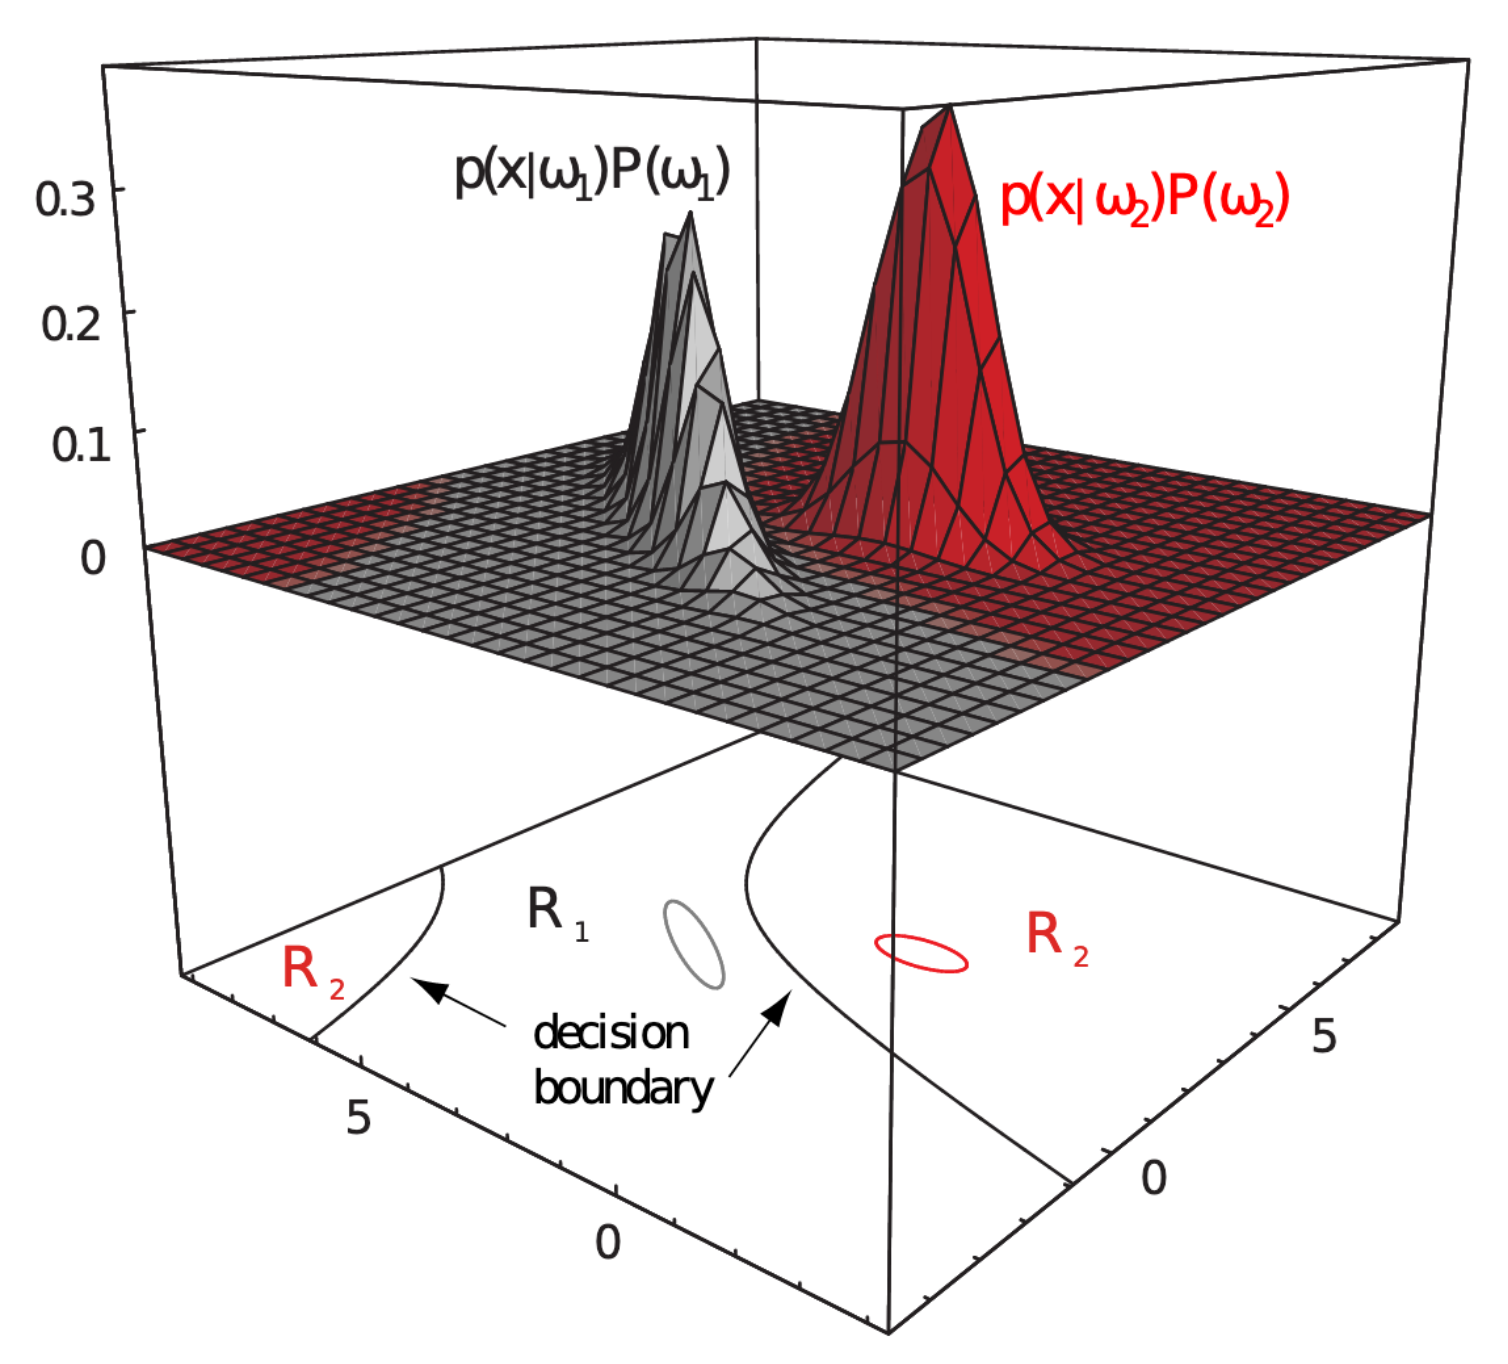
\includegraphics[width=0.8\linewidth]{BayesDecisionRuleFig1}
	\caption{Example of classifiers.}
	\label{fig:BayesDecisionRuleFig1}
\end{figure}
Let's first recall the equation for the multivariate normal density:
\begin{center}
	$\displaystyle p(\vect{x};\mu,\Sigma)=\cfrac{1}{(2\pi)^{\myfrac{d}{2}}\abs{\Sigma}^{\myfrac{1}{2}}}e^{-\frac{1}{2}(\vect{x}-\vect{\mu})^T\Sigma^{-1}(\vect{x}-\vect{\mu})}$
\end{center}
And let's remember that the covariance matrix $\Sigma$ is always symmetric and positive semi-definite, and becomes strictly positive if the dimension of the feature space is $f$.\newline
This distribution can map the probability of $\vect{x}$ given $\vect{y}_i$:
\begin{center}
	$\displaystyle p(\vect{x}\vert y_i)=\cfrac{1}{(2\pi)^{\myfrac{d}{2}}\abs{\Sigma_i}^{\myfrac{1}{2}}}e^{-\frac{1}{2}(\vect{x}-\vect{\mu}_i)^T\Sigma^{-1}(\vect{x}-\vect{\mu}_i)}$
\end{center}
Given a multivariate normal distribution, the location of points of constant density are hyper-ellipsoids of constant Mahalanobis distance (Equation~\ref{eq:MahalanobisDistance}) from $\vect{x}$ to $\vect{\mu}$. \newline
%
%
\subsection{Discriminant function}
Let's know take expression from before describing discriminant functions:
\begin{center}
	$\displaystyle g(x)=\ln{P(x\vert y_i)}+\ln{P(y_i)}$
\end{center}
And substitute the multivariate normal distribution inside:
\begin{center}
	$\displaystyle g_i(\vect{x})=\ln{\cfrac{1}{(2\pi)^{\frac{d}{2}}\abs{\Sigma}^\frac{1}{2}}e^{-\frac{1}{2}(\vect{x}-\vect{\mu}_i)^T\Sigma_i^{-1}(\vect{x}-\vect{\mu}_i)}}+\ln{P(y_i)}$\\
	
	$\displaystyle g_i(\vect{x})=\ln{\left[\cfrac{1}{(2\pi)^{\frac{d}{2}}\abs{\Sigma}^\frac{1}{2}}\right]}+\left[-\cfrac{1}{2}(\vect{x}-\vect{\mu}_i)^T\Sigma^{-1}(\vect{x}-\vect{\mu}_i) \right]+\ln{P(y_i)}$\\
	
	$\displaystyle g_i(\vect{x})=-\frac{d}{2}\ln{2\pi}-\frac{1}{2}\ln{\abs{\Sigma_i}}-\cfrac{1}{2}(\vect{x}-\vect{\mu}_i)^T\Sigma^{-1}(\vect{x}-\vect{\mu}_i)+\ln{P(y_i)}$
\end{center}
Since  $\frac-{d}{2}ln2\pi$ does not depend on $i$ then we can erase it:
\begin{equation}
	g_i(\vect{x})=-\frac{1}{2}\ln{\abs{\Sigma_i}}-\cfrac{1}{2}(\vect{x}-\vect{\mu}_i)^T\Sigma^{-1}(\vect{x}-\vect{\mu}_i)+\ln{P(y_i)}
	\label{eq:DiscriminantFunction}
\end{equation}
%
\subsubsection{$\Sigma_i=\sigma^2I$}
All features are statistically independent which means that they have the same variance $\sigma^2$. \newline
Now the covariance determinant $\abs{\Sigma_i}=\sigma^{2d}$ is independent of $i$ and can hence be ignored from the Equation~\ref{eq:DiscriminantFunction}.\newline
The inverse of the covariance is $\Sigma^{-1}_i=(\myfrac{1}{\sigma^2})I$ and even though is not dependent of $i$, it cannot be cancelled because part of another term.
The new discriminant functions become:
\begin{center}
	$\displaystyle g_i(\vect{x})=-\frac{1}{2}(\vect{x}-\vect{\mu}_i)^T\frac{I}{\sigma^2}(\vect{x}-\vect{\mu}_i)+\ln{P(y_i)}$
\end{center}
Which equals to:
\begin{center}
	$\displaystyle g_i(\vect{x})=-\cfrac{\abs{\abs{\vect{x}-\vect{\mu}_i}}^2}{2\sigma^2}+\ln{P(y_i)}$
\end{center}
Expanding the quadratic term, we obtain:
\begin{center}
	$\displaystyle g_i(\vect{x})=-\cfrac{1}{2\sigma^2}\left[\vect{x}^T\vect{x}-2\vect{\mu}^T_i\vect{x}+\vect{\mu}^T_i\vect{\mu}_i\right]+\ln{P(y_i)}$
\end{center}
Discarding terms which are independent of $i$ we obtain \textit{linear discriminant functions}:
\begin{equation}
	g_i(\vect{x})=
	\underbrace{\frac{1}{\sigma^2}\vect{\mu}^T_i    \rule[-12pt]{0pt}{5pt}}_{\mbox{$\vect{w}_{i}^T$}}\vect{x}
	-\underbrace{-\frac{1}{2\sigma^2}\vect{\mu}^T_i\vect{\mu}_i+\ln{P(y_i)} \rule[-12pt]{0pt}{5pt}}_{\mbox{$w_{i0}$}}
\end{equation}
This is in fact linear: said $\vect{w}_i^T=\myfrac{1}{\sigma^2}\vect{\mu}_i^T\vect{x}$ and $w_{i0}=-\myfrac{1}{2\sigma^2}\vect{\mu}^T_i\vect{\mu}_i+\ln{P(y_i)}$, none of them depend on $\vect{x}$, hence $g_i(\vect{x})$ can be rewritten has:
\begin{center}
	$\displaystyle g_i(\vect{x})=\vect{w}_i^T\vect{x}+w_{i0}$
\end{center}
which is indeed a line. \newline
We have said that the boundaries are the region where the discriminant functions intersect, that is when they are equal $g_i(\vect{x)}=g_j(\vect{x})$. It's possible to find the equation of the decision boundaries:
\begin{center}
	$\displaystyle g_i(\vect{x})=g_j(\vect{x})$\\
	$\displaystyle \cfrac{\vect{\mu}_i^T\vect{x}}{\sigma^2}-\frac{\vect{\mu}_i^T\vect{\mu}_i}{2\sigma^2}+\ln{P(y_i)}= \frac{\vect{\mu}_j^t\vect{x}}{\sigma^2}-\frac{\vect{\mu}_j^t\vect{\mu}_j}{2\sigma^2}+\ln{P(y_j)}$\\
\end{center}
\begin{equation}
	\underbrace{\frac{(\vect{\mu}_i-\vect{\mu}_j)^T}{\sigma^2}\rule[-12pt]{0pt}{5pt}}_{\mbox{$\vect{w}^T$}}
	\vect{x}
	\underbrace{-\frac{\vect{\mu}_i\vect{\mu}_j}{\sigma^2}+\frac{\vect{\mu}_j^t\vect{\mu}_j}{\sigma^2}+\ln{\frac{P(y_i)}{P(y_j)}}\rule[-12pt]{0pt}{5pt}}_{\mbox{$\vect{x}_0$}}
	=0
\end{equation}
Which do not depend on $\vect{x}$ again hence making it linear again:
\begin{center}
	$\displaystyle \vect{w}^T\vect{x}+\vect{x}_0$
\end{center}
This line (which is an hyperplane btw) is orthogonal to the vector $\vect{w}$, that is to the distance between $\vect{\mu}_i$ and $\vect{\mu}_j$ since $\vect{w}$ is transposed with respect to $\vect{x}$.\newline
Moreover the hyperplane passes through $\vect{x}_0$ which is based on the prior probabilities of classed being equal. If they are, then $\vect{x}_0$ is halfway between the means, while if they are not, $\vect{x}_0$ shifts away from the more likely mean. This can be seen in the logarithm: if $y_i=y_j$, then it would be $\ln{1}=0$.\newline
\begin{figure}[htp]
	\begin{minipage}{\linewidth}
		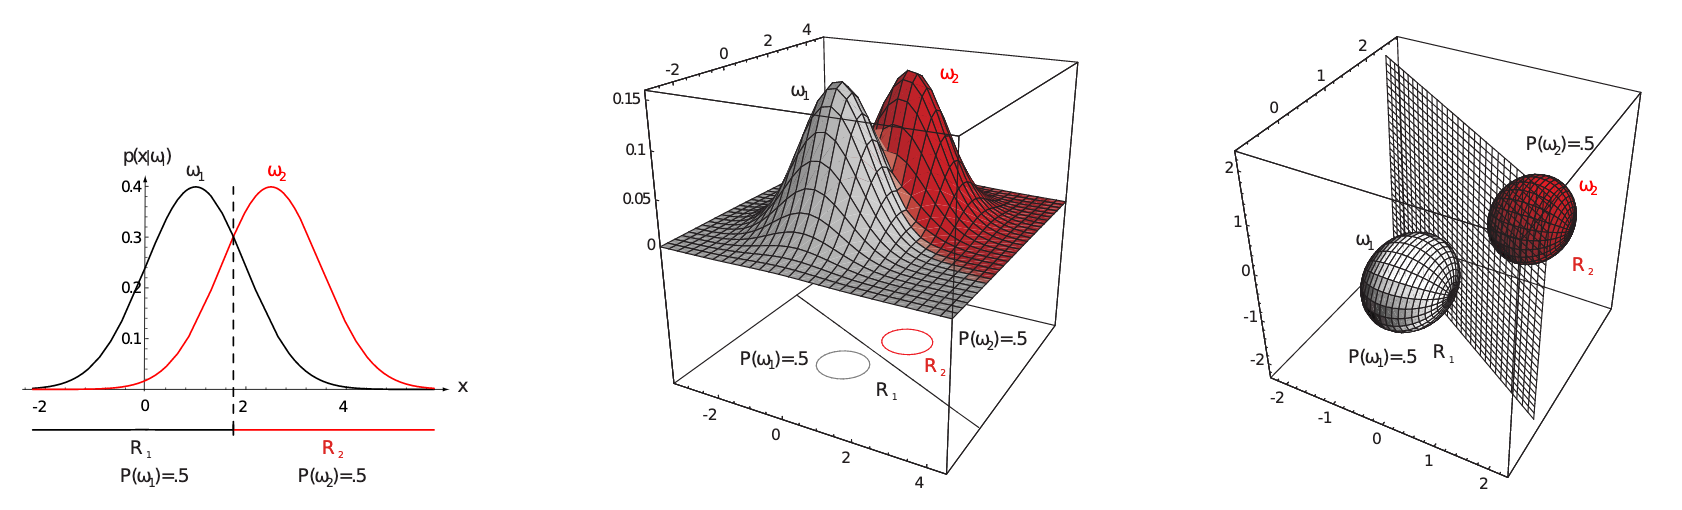
\includegraphics[width=0.9\linewidth]{BayesDiscriminantFunctions1}
		\caption{Case in which $P(y_i)=P(y_j)$. The discriminant function is a line which pass right through the middle of the distance of the two regions.}
	\end{minipage}
\end{figure}\\
\begin{figure}[htp]
	\begin{minipage}{\linewidth}
		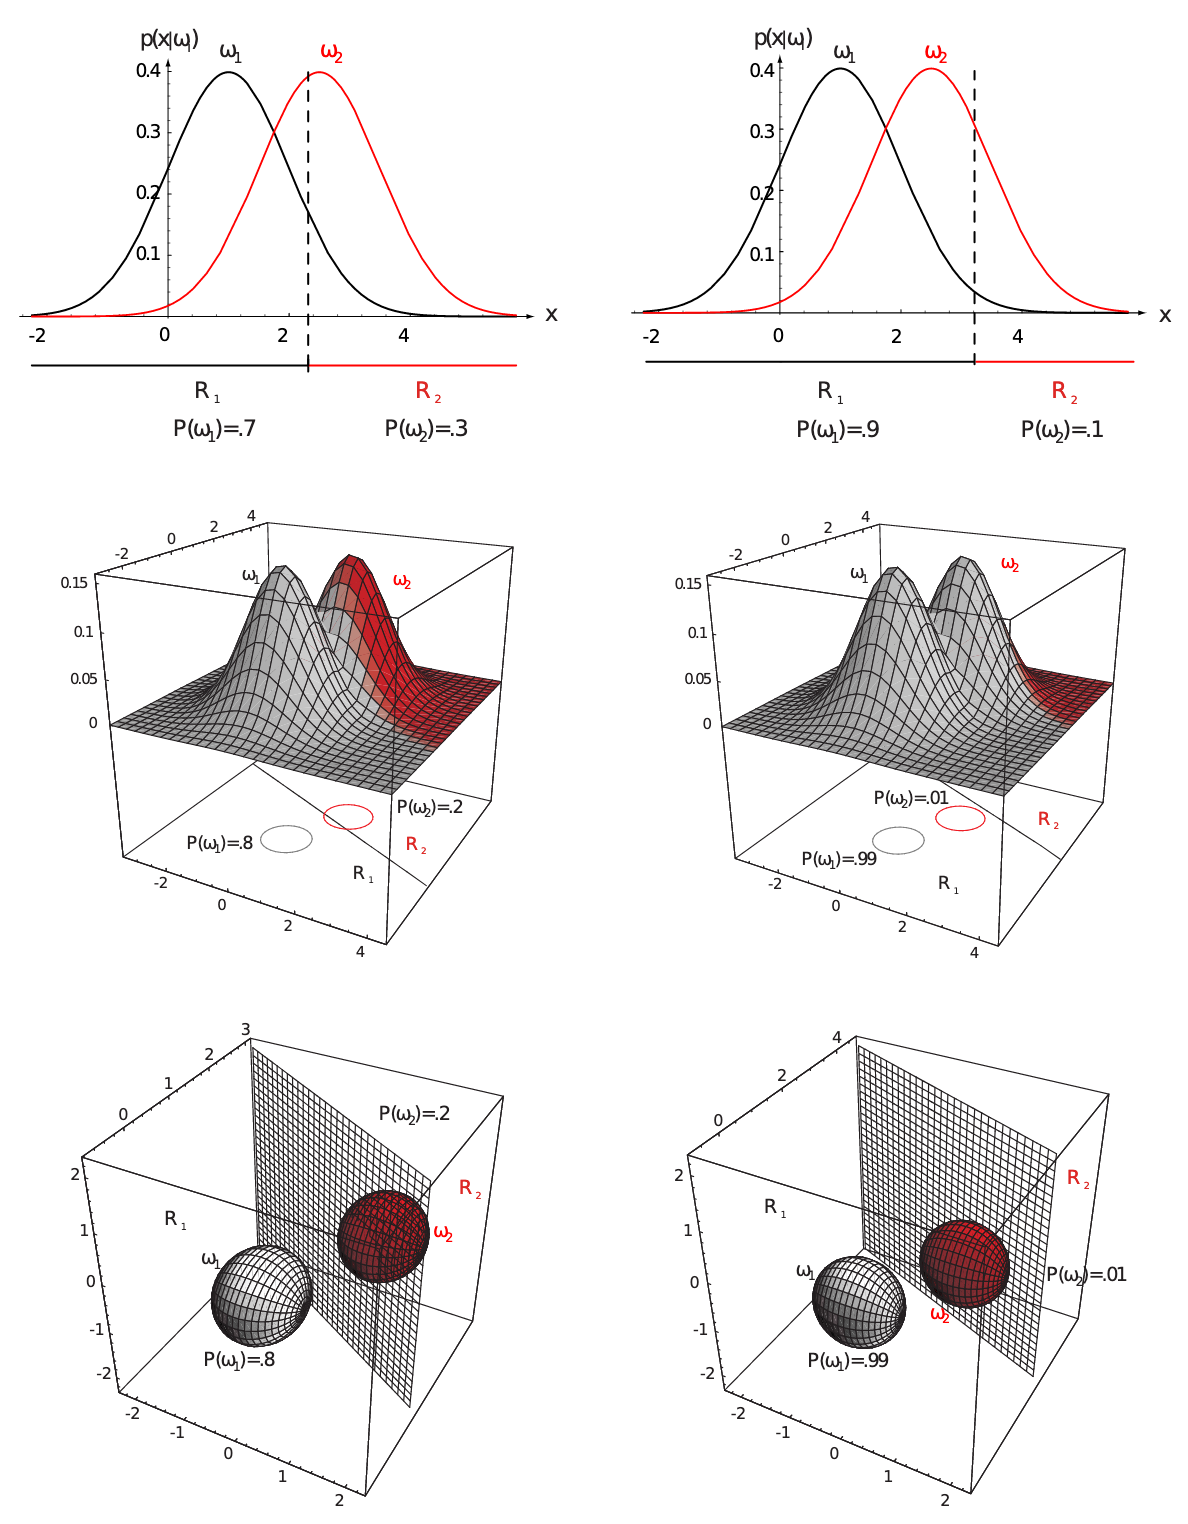
\includegraphics[width=0.9\linewidth]{BayesDiscriminantFunctions2}
		\caption{Case in which $P(y_i)\neq P(y_j)$. It's possible to notice that the more the probability difference increases, the more the line drifts away from that probability.}
	\end{minipage}
\end{figure}
%TODO check if missing something in the appendix